\documentclass[a4paper,11pt]{article}

\usepackage{lipsum}
\usepackage[english]{babel}
\usepackage[margin=20mm]{geometry}
\usepackage{graphicx}
\usepackage{subfigure}

\title{Multi-Agent Systems Summative Assignment}
\date{\today}
\author{James King}

\begin{document}
\maketitle

\section{Problem Specification}
\subsection{Overview}
\subsubsection{World}
The task is a simple turn-based game within a tile based world, where two or more teams of bots compete for survival. Each team starts with one or more \emph{home} tiles, upon which a bot belonging to that team begins. Every remaining tile in the world may be a solid \emph{wall}, a \emph{resource} item, a \emph{bot}, or \emph{empty}. The world is a two dimensional grid of fixed dimensions, and has the topology of the surface of a torus (travelling off one side of the grid will bring you to the opposite side). The world is initially unknown to players of the game, but at the start of each turn every player is given the state of previously undiscovered tiles that are within a certain fixed \emph{vision radius} of any agent on their team. The locations of resources, along with the positions, team affiliation and direction of agents within the vision radius is also given before each turn.

\subsubsection{Bots}

Bots have a \emph{direction} property, which may be any one of the cardinal directions (\emph{north}, \emph{east}, \emph{south}, or \emph{west}). Each turn, each team decides a single action to perform with each bot belonging to them. This action may be to rotate the bot \emph{left} or \emph{right} (so a bot that was facing east which turns left will now face north), to \emph{move} one tile in the direction it is currently facing (unless a wall is in the destination tile, in which case it does not move), or to \emph{pass} and do nothing. After each team decides on a set of moves, all the bots commit to their assigned instruction simultaneously. If any two or more bots occupy the same tile they are removed from the world before the next turn. Also, a bot is removed if it is neighbouring another bot of a different team that is facing it.

\begin{figure}[ht]
  \centering
  \mbox{
    \subfigure
      [The purple bot moves to eliminate the pink bot.]
      {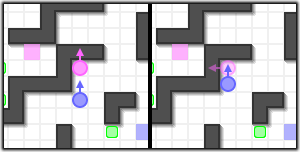
\includegraphics[width=0.45\linewidth]{kill}}
    \quad
    \subfigure
      [Mutual elimination when two bots occupy the same tile.]
      {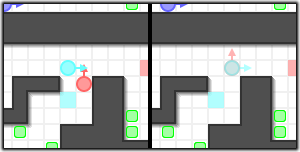
\includegraphics[width=0.45\linewidth]{mutual}}
  }
  \caption{Demonstrations of the two rules for bot elimination.}
\end{figure}

\subsubsection{Resources}

Resources are items that appear at regular intervals in the world on randomly selected empty tiles. These are initially stationary, but if a bot appears on a neighbouring tile and faces the resource, the bot begins to \emph{carry} the resource which will attempt to remain one tile in front of the carrying bot. If the carrying bot moves forward, the resource is \emph{pushed} in the direction the bot moved by one tile. If the bot turns, the resource will move to whichever tile the bot is now facing. However, if the destination tile for the resource when either pushed or turned isn't vacant, the resource is removed from the world. Finally, if the resource is moved to a home tile, a new bot belonging to the home tile's corresponding team is created in its place.

\begin{figure}[ht]
  \centering
  \mbox{
    \subfigure
      [Moving a resource (green) onto a home tile spawns a new bot and consumes the resource.]
      {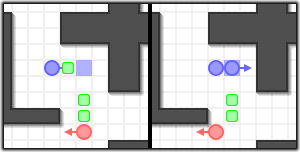
\includegraphics[width=0.45\linewidth]{capture}}
    \quad
    \subfigure
      [Pushing a resource into a wall, bot, or another resource will remove it.]
      {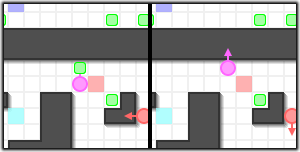
\includegraphics[width=0.45\linewidth]{destroy}}
  }
  \caption{Demonstrations of resource consumption and destruction.}
\end{figure}

\subsubsection{Win Condition \& Goals}

The game lasts until either a predetermined turn limit is reached, or only bots belonging to one team remain. When the game ends, whichever team has the most remaining bots is declared the winner. The aim of the game is therefore to try and eliminate as many bots belonging to opposing teams as possible, while attempting to transport resources back to a home tile owned by your team and preventing other teams from doing so. 

\end{document}
